\documentclass[11pt]{article}
\usepackage[T1]{fontenc}
\usepackage{lmodern,amsmath,amssymb,amsthm,mathtools,microtype,booktabs}
\usepackage[margin=1in]{geometry}
\usepackage{xcolor,graphicx,xurl}
\usepackage[colorlinks=true,linkcolor=blue!50!black,citecolor=blue!50!black,urlcolor=blue!50!black]{hyperref}
\newtheorem{theorem}{Theorem}[section]
\newtheorem{lemma}[theorem]{Lemma}
\newtheorem{proposition}[theorem]{Proposition}
\newtheorem{corollary}[theorem]{Corollary}
\theoremstyle{remark}\newtheorem{remark}[theorem]{Remark}
\newcommand{\E}{\mathbb E}
\newcommand{\Pp}{\mathbb P}
\newcommand{\C}{\mathbb C}
\newcommand{\Z}{\mathbb Z}
\newcommand{\N}{\mathbb N}
\newcommand{\abs}[1]{\left|#1\right|}
\newcommand{\norm}[1]{\left\|#1\right\|}
\newcommand{\one}{\mathbf 1}
\newcommand{\DGRH}{\textup{DGRH}}
\DeclareMathOperator{\ord}{ord}
\DeclareMathOperator{\supp}{supp}
\setlength{\emergencystretch}{3em}
\title{Every sparse prime-product transition is compound Poisson\\[4pt]\large Bounded quotients, a sharp mixing criterion, and a uniform finite-population correction}
\author{Research note for the ProveIt project}
\date{27 November 2026}
\begin{document}
\maketitle
\begin{abstract}
Assume the generalized Riemann hypothesis for Dirichlet $L$-functions. Retain an arbitrary fixed positive fraction $a$ of the primes at most $C\log^2q$, and choose a prescribed number of distinct retained primes. Write $m$ for the retained population and $h$ for the smaller of the chosen and omitted cardinalities. In the sparse regime $B\log q\le h=o(m)$, we classify every subsequential product-residue profile on the normalized pointwise scale. After passage to a quotient of order at most $\lfloor1/a\rfloor$ and a deterministic phase correction, every surviving profile is compound Poisson. Conversely, every such finite-group compound-Poisson profile is realized by retained prime sets. Equidistribution holds precisely when $h/m$ times the least distance from a fibre of a nonprincipal character of order at most $\lfloor1/a\rfloor$ tends to infinity. The finite probability argument gives an explicit signed-measure expansion through order $1/h$, with a uniform $O(h^{-2})$ remainder in a bounded critical window. The bounded-quotient reduction is inherited from the supplied article; the contributions proposed here are the all-density limit classification, criterion, and group-valued correction. Historical priority is not certified.
\end{abstract}

\section{Source analysis, dependencies, and the new question}

This note uses the ProveIt materials at the pinned revision
\begin{center}\small\texttt{6d284fcf75bc3a91bb2e79ba7636f94724bff62c}.\end{center}
The project README describes an article merging 142 reports, together with 42 further placed reports awaiting merger. The pinned tree also contains ten further incoming archives. It explicitly distinguishes the imported GRH theorem, downstream proofs, and formalization status \cite{repo,article}. The relevant mathematical predecessor is the article's section \texttt{dir.tex}, especially the labels
\texttt{dir:lem:bias}, \texttt{dir:thm:quotient},
\texttt{dir:thm:disjoint-growing}, and
\texttt{dir:thm:disjoint-mixing}.

The article already reduces fixed-quota prime-product laws, at every fixed positive retained density, to a quotient of bounded order. It also gives quadratic and cubic mixing criteria above retained density $1/4$, including several disjoint products. The separate quadratic-fibre report proves a sharper one-mode approximation above density $1/3$ and its scalar first finite-population correction \cite{quadratic}. The incoming quarter-density report also gives exact support and coverage criteria for $C_4$ and $C_2\times C_2$, together with an independent-exception coupling bound $t(t-1)/(2m)$ in total variation \cite{quarter}. None of these existing statements is claimed as new here.

The additional question is what \emph{all} sparse-quota transition profiles look like, including below density $1/4$, where cyclic groups of order four and products of quadratic quotients occur. We answer it by a complete subsequential classification, a converse realization theorem, and a uniform group-algebra expansion. The analytic arithmetic input is only
\[
 \DGRH:\quad \Re\rho=\tfrac12
 \quad\text{for every nontrivial zero of every Dirichlet $L$-function}.
\]
We treat the supplied theorem as an input, as the merged article does; we have not rerun its full Lean build. The present theorems are ordinary mathematical proofs, not new Lean-checked declarations. No simplicity or linear-independence hypothesis on zeros, and no non-Dirichlet GRH, is used.

The finite probability lemmas in Sections~\ref{sec:decay}--\ref{sec:expansion} are unconditional. The arithmetic applications use a standard smoothed explicit formula, together with finite Fourier analysis. Basic Poisson approximation and limit laws for infinitesimal arrays are classical. Our proposed research contribution is the exact combination of an arbitrary-density arithmetic classification on the normalized pointwise scale, its bounded-order fibre criterion, and the stated uniform signed-measure correction. The literature comparison in Section~\ref{sec:comparison} is targeted rather than exhaustive.

\section{Main arithmetic statements}\label{sec:main}

Fix $0<a\le1$, put $D=\lfloor1/a\rfloor$, and let
\[
 G_q=(\Z/q\Z)^\times,\quad L=\log q,\quad
 \mathcal P_q=\{p\le CL^2:p\text{ prime},\ p\nmid q\},\quad N=|\mathcal P_q|.
\]
Let $S\subseteq\mathcal P_q$ have $m\ge aN$ elements. Distinct primes are distinct population labels even when their residues coincide. For $1\le k<m$, let $X_k$ be the product in $G_q$ of a uniformly chosen $k$-element subset of $S$. Thus
\[
 R_{S,k}(g)=\binom mk\Pp(X_k=g)
\]
counts squarefree products with exactly $k$ prime factors from $S$ and residue $g$. Put
\[
 h=\min(k,m-k),\qquad u=h/m,\qquad U_S=\prod_{p\in S}p\pmod q.
\]
The variable
\begin{equation}\label{eq:Y}
 Y=\begin{cases}X_k,&k\le m/2,\\ U_SX_k^{-1},&k>m/2\end{cases}
\end{equation}
has the distribution of the product of a uniform $h$-subset. Translation and inversion preserve discrepancy from uniform.

For every nonprincipal character $\chi$ of order at most $D$, define its fibre distance by
\[
 t_\chi(S)=m-\max_{\zeta\in\chi(G_q)}\#\{p\in S:\chi(p)=\zeta\},\qquad
 T_D(S)=\min_{1<\ord\chi\le D}t_\chi(S).
\]
An empty minimum is $+\infty$. Define the normalized pointwise discrepancy
\[
 \Delta_{S,k}=\max_{g\in G_q}\abs{\frac{\varphi(q)R_{S,k}(g)}{\binom mk}-1}.
\]

\begin{theorem}[Sharp mixing criterion at every fixed density; uses DGRH]\label{thm:criterion}
For every $0<a\le1$ and $A>0$ there are constants $B,C>0$ such that the following holds along any sequence $q\to\infty$ with $m\ge aN$, $h\ge B\log q$, and $h/m\to0$:
\begin{equation}\label{eq:iff}
 \Delta_{S,k}\longrightarrow0
 \quad\Longleftrightarrow\quad
 \frac{hT_D(S)}m\longrightarrow+\infty.
\end{equation}
For $D\ge2$, there is $c_D>0$ depending only on $D$ such that, without needing $h/m\to0$ for the upper bound,
\begin{equation}\label{eq:upper}
 \Delta_{S,k}\le20(D-1)\exp\left(-c_D\frac{hT_D(S)}m\right)+q^{-A}.
\end{equation}
For $D=1$, one has $\Delta_{S,k}\le q^{-A}$.
\end{theorem}

To state the full transition classification, use multiplicative notation for a finite abelian group $F$, whose identity is $e$. For rates $\lambda_x\ge0$ indexed by $x\ne e$, let $J_x$ be independent Poisson variables of means $\lambda_x$, and define
\begin{equation}\label{eq:CP}
 P_\Lambda=\mathcal L\left(\prod_{x\ne e}x^{J_x}\right),\qquad
 \Lambda=\sum_{x\ne e}\lambda_x(\delta_x-\delta_e).
\end{equation}
Equivalently $P_\Lambda=\exp_*(\Lambda)$, where the exponential is taken in the convolution algebra of signed measures. Its Fourier transform is
\begin{equation}\label{eq:CPfourier}
 \widehat P_\Lambda(\chi)
 =\exp\left(\sum_{x\ne e}\lambda_x(\chi(x)-1)\right).
\end{equation}

\begin{theorem}[Complete sparse-quota classification; uses DGRH]\label{thm:classification}
The constants $B,C$ in Theorem~\ref{thm:criterion} may be chosen so that the following holds. Every sequence $q_n\to\infty$, $m_n\ge aN_n$, $h_n\ge B\log q_n$, and $h_n/m_n\to0$ has a subsequence on which there exist:
\begin{itemize}
\item a fixed finite abelian group $F$ with $|F|\le D$;
\item surjective homomorphisms $\pi_n:G_{q_n}\to F$ and phases $b_n\in F$;
\item finite nonnegative rates $\lambda_x$ for $x\in F\setminus\{e\}$;
\end{itemize}
such that
\begin{equation}\label{eq:classification}
 \max_{g\in G_{q_n}}
 \abs{|G_{q_n}|\Pp(Y_n=g)
       -|F|P_\Lambda\bigl(\pi_n(g)b_n^{-h_n}\bigr)}\longrightarrow0.
\end{equation}
Conversely, every compound-Poisson law on every finite abelian group $F$ with $|F|\le D$ occurs in this way, for some sequence of moduli and retained prime sets, with $h_n=\lceil B\log q_n\rceil$.
\end{theorem}

The normalization in \eqref{eq:classification} is essential. Each residue probability is typically of order $1/\varphi(q)$; the theorem resolves its relative profile. It is stronger than convergence of a projected law alone or an unnormalized error tending to zero. The limiting quotient is allowed to vary before taking a subsequence; there is no claim that one quotient works for all possible retained sets.

Every Fourier coefficient in \eqref{eq:CPfourier} is nonzero. Thus a compound-Poisson law on a nontrivial finite group is never exactly uniform. Its support is the subgroup generated by the jumps with positive rates: in a finite group, the semigroup generated by these jumps is their subgroup. A profile may therefore have limiting holes even when a few finite-population exceptions make the exact support larger.

\section{The analytic input and the bounded quotient}\label{sec:quotient}

We include proofs to make the dependence on the article's existing reduction explicit.

\begin{lemma}[Endpoint small bias; uses DGRH]\label{lem:bias}
For every $\epsilon>0$ there is $C>0$ such that, for all sufficiently large $q$,
\[
 N\sim\frac{C\log^2q}{\log(C\log^2q)},\qquad
 \max_{\chi\ne1}\abs{\frac1N\sum_{p\in\mathcal P_q}\chi(p)}\le\epsilon.
\]
The maximum is over all nonprincipal Dirichlet characters modulo $q$.
\end{lemma}
\begin{proof}
Write $y=C\log^2q$. Fix $0<\eta<1/4$, and choose a fixed smooth $W$ supported in $(0,1)$ with $0\le W\le1$ and $W=1$ on $[\eta,1-\eta]$. Mellin inversion of $-L'/L$, shifted from real part $2$ to $1/4$, gives for a primitive nonprincipal character $\psi$ of conductor $f$ the smoothed explicit formula
\[
 \sum_{n\ge1}\Lambda(n)\psi(n)W(n/y)
 =-\sum_\rho y^\rho\widetilde W(\rho)
       +O_W(y^{1/4}\log(2f)).
\]
Here $\widetilde W(s)=\int_0^\infty W(v)v^{s-1}\,dv$, and zeros are counted with multiplicity. The standard analytic facts used in this contour shift are the functional equation, the local logarithmic-derivative bound away from zeros, and the bound $O(\log(2f(2+|T|)))$ for the number of zeros in a unit strip; see \cite[Chs.~10, 12--13]{MV}. The Mellin transform decays faster than every inverse power of $|\Im s|$ on the relevant fixed strip. Under DGRH the new vertical line stays distance $1/4$ from every nontrivial zero, and horizontal contours can be chosen to avoid zero ordinates. The zero sum is consequently $O_W(\sqrt y\log(2f))$.

Remove prime powers at cost $O(\sqrt y\log^2y)$. Replacing $\psi$ by the induced character modulo $q$ changes the weighted prime sum only at primes dividing $q$, with total weight at most $\log q$. Thus, uniformly in every nonprincipal $\chi$ modulo $q$,
\[
 \abs{\sum_{p\in\mathcal P_q}\chi(p)(\log p)W(p/y)}
 \ll_W\sqrt y\log(2q)+\sqrt y\log^2y+\log q.
\]
The ordinary prime number theorem shows that restoring $W$ to one costs at most $(2\eta+o(1))y$, and replacing $\log p$ by $\log y$ costs at most
$\pi(y)\log y-\vartheta(y)=o(y)$. At most $\log q/\log2$ primes divide $q$, so $N\log y\sim y$. Division by this quantity yields a normalized bound
\[
 2\eta+O_W(C^{-1/2})+o(1).
\]
Choose $\eta$ first and then $C$. The onset is uniform in $\chi$ and $q$ for these fixed choices.
\end{proof}

\begin{lemma}[Few almost-constant characters]\label{lem:gram}
Let a labelled pool $P$ in a finite abelian group have nonprincipal character means of modulus at most $\epsilon$. Let $S\subseteq P$ have $|S|/|P|\ge a$. There are $\tau,\epsilon>0$ depending only on $a$ such that the subgroup $H$ generated by the characters whose mean on $S$ has modulus greater than $1-\tau$ has order at most $D=\lfloor1/a\rfloor$.
\end{lemma}
\begin{proof}
Use normalized counting measure on $P$. Any $r$ distinct character vectors have Gram matrix with diagonal entries $1$ and off-diagonal moduli at most $\epsilon$, hence operator norm at most $1+(r-1)\epsilon$. Put $\alpha=|S|/|P|$. If their biases on $S$ are all at least $v$, applying the Gram bound to $\one_S$ gives
\[
 r\alpha^2v^2\le\alpha(1+(r-1)\epsilon),\qquad
 r\le\frac{1-\epsilon}{a v^2-\epsilon}
\]
when the denominator is positive.

A character of bias greater than $1-\tau$ has normalized $L^2(S)$ distance less than $\sqrt{2\tau}$ from a unit complex constant. Its inverse has the same property. By telescoping, a product of at most $D$ such generators and inverses has distance at most $D\sqrt{2\tau}$ from a unit constant, hence bias at least $1-D^2\tau$. Because $D+1>1/a$, choose $\tau$ and then $\epsilon$ so that
\[
 \frac{1-\epsilon}{a(1-D^2\tau)^2-\epsilon}<D+1
\]
with positive denominator. The word ball of radius $D$ in $H$ then has at most $D$ elements. If $|H|\ge D+1$, word balls starting from the identity gain at least one new element at every radius until exhausting $H$, so the radius-$D$ ball would have at least $D+1$ elements. This contradiction proves the claim.
\end{proof}

\begin{lemma}[Fixed-quota coefficient estimate]\label{lem:circle}
For $|z_j|=1$, $1\le h\le m/2$, and $v=|m^{-1}\sum_jz_j|$,
\[
 \abs{\binom mh^{-1}[w^h]\prod_{j=1}^m(1+wz_j)}
 \le(m+1)\exp(-(1-v)h/2).
\]
\end{lemma}
\begin{proof}
On $|w|=r=h/(m-h)$ use
\[
 \frac{|1+re^{i\theta}z_j|^2}{(1+r)^2}
 =1-\frac{2r(1-\Re(e^{i\theta}z_j))}{(1+r)^2}.
\]
Multiply the inequality $1-x\le e^{-x}$ and take square roots. The product is at most
$(1+r)^m\exp(-rm(1-v)/(1+r)^2)$. Cauchy's coefficient bound contributes the factor $(1+r)^m/(r^h\binom mh)$, the reciprocal of the binomial $(m,h/m)$ mass at its integer mean $h$. That mean is a mode, so its mass is at least $1/(m+1)$. Finally $rm/(1+r)^2=h(m-h)/m\ge h/2$.
\end{proof}

\begin{proposition}[Inherited quotient reduction; uses DGRH]\label{prop:quotient}
Fix $a>0$ and $A>0$. For suitable $B,C>0$, all sufficiently large $q$, every retained set of density at least $a$, and $h\ge B\log q$, there are a subgroup $H\le\widehat G_q$ of order $d\le D$ and a quotient $\pi:G_q\to E=\widehat H$ such that
\begin{equation}\label{eq:reduction}
 \max_g\abs{|G_q|\Pp(Y=g)-d\Pp(\pi(Y)=\pi(g))}\le q^{-A}.
\end{equation}
\end{proposition}
\begin{proof}
Apply Lemmas~\ref{lem:bias} and \ref{lem:gram}. Every character outside $H$ has retained-set bias at most $1-\tau$. Its $h$-subset coefficient is at most $(m+1)e^{-\tau h/2}$ by Lemma~\ref{lem:circle}. Fourier inversion splits into the sum over $H$, exactly $d$ times the quotient probability, and a remainder at most $|G_q|(m+1)e^{-\tau h/2}$. Since $|G_q|\le q$, $m\le C\log^2q$, and $h\ge B\log q$, this remainder is at most $q^{-A}$ for large $q$ upon choosing $B$ sufficiently large.
\end{proof}

\section{Finite-order Fourier decay without a growing prefactor}\label{sec:decay}

The next estimate lets the relevant minority scale tend to infinity arbitrarily slowly. A factor $\sqrt h$ or $m$ in front of the exponential would not suffice for that purpose.

\begin{lemma}[Split-pair decay]\label{lem:pair}
Let $z_1,\ldots,z_m$ be roots of unity of order dividing $d$, where $2\le d\le D$. Put
\[
 t=m-\max_\zeta\#\{j:z_j=\zeta\},\qquad 1\le h\le m/2.
\]
If $E_h$ is the expected product over a uniform $h$-subset, then
\begin{equation}\label{eq:pair}
 |E_h|\le20\exp(-c_Dht/m),\qquad
 c_D=\frac{1-\cos(\pi/D)}{\max(D,8)}.
\end{equation}
\end{lemma}
\begin{proof}
For $m<8$, the asserted bound follows from $|E_h|\le1$; enlarge no constants. Suppose $m\ge8$. A largest value class has size $n_{\max}\ge m/D$. Pair
\[
 r=\min(n_{\max},t,\lfloor m/4\rfloor)\ge t/\max(D,8)
\]
of its labels with distinct labels of different values. At least $m/2$ labels remain unpaired. Conditional on the selected count in every pair and the selected unpaired labels, orientations of split pairs are independent fair choices. For different $d$th roots $z,z'$,
\[
 \left|\frac{z+z'}2\right|\le\cos(\pi/d)\le\kappa:=\cos(\pi/D).
\]
It follows that $|E_h|\le\E(\kappa^Z)$, where $Z$ is the number of split pairs in the uniform $h$-subset.

Generate the subset by independent Bernoulli$(u)$ selection of all labels, $u=h/m$, conditioned on total count $B_m=h$. Tilt the independent law by the nonnegative weight $\kappa^Z$. Its normalizing constant is
\[
 \E\kappa^Z=(1-2(1-\kappa)u(1-u))^r.
\]
Even when $\kappa=0$, this tilt is well-defined, because the event of no split pairs has positive probability. Under the tilt the unpaired labels remain independent Bernoulli$(u)$, independent of all pairs. Hence
\[
 \E(\kappa^Z\mid B_m=h)
 =\E\kappa^Z\frac{\Pp_{\rm tilt}(B_m=h)}{\Pp(B_m=h)}.
\]
The denominator is at least $3/(20\sqrt h)$: the integer mean $h$ is a mode, while Chebyshev places at least $3/4$ of the mass in an interval containing at most $5\sqrt h$ integers. With $n=m-2r\ge m/2$, Fourier inversion gives
\begin{align*}
 \sup_j\Pp(\operatorname{Bin}(n,u)=j)
 &\le\frac1{2\pi}\int_{-\pi}^{\pi}
       e^{-2nu(1-u)\sin^2(\theta/2)}\,d\theta\\
 &\le\frac{\sqrt\pi}{2\sqrt{2nu(1-u)}}
 \le\frac{\sqrt\pi}{\sqrt{2h}}.
\end{align*}
The tilted total is the sum of this unpaired binomial and an independent variable, so its atom is at most the same bound. The atom ratio is less than $20$. Finally $u\le1/2$ gives
\[
 (1-2(1-\kappa)u(1-u))^r
 \le e^{-(1-\kappa)ur}
 \le e^{-c_Dut}.
\]
This proves \eqref{eq:pair}.
\end{proof}

\section{A uniform group-valued finite-population expansion}\label{sec:expansion}

Let $F$ be a finite abelian group. For signed measures use convolution $*$ and the norm
$\|\mu\|_1=\sum_{x\in F}|\mu(x)|$. A probability measure has norm one, convolution is submultiplicative, and total variation distance is half this norm of the difference.

Consider a population of $m-t$ identity labels and $t$ labelled defects $x_1,\ldots,x_t\ne e$. Let $\mu_{m,h}$ be the law of its product over a uniform $h$-subset. Assume $1\le h\le m/2$ and $0\le t\le m/2$, and put $u=h/m$, $\lambda=ut$. Define the polynomial probability law
\begin{equation}\label{eq:nu}
 \nu(v)=\mathop{*}_{i=1}^t\bigl(\delta_e+v(\delta_{x_i}-\delta_e)\bigr),\qquad0\le v\le1.
\end{equation}
Thus $\nu(u)$ includes each defect independently with probability $u$, whereas $\mu_{m,h}$ respects the fixed population quota. Derivatives of $\nu$ mean ordinary polynomial derivatives in the vector space of signed measures.

\begin{theorem}[Uniform second-order correction; unconditional]\label{thm:expansion}
In the preceding setup,
\begin{equation}\label{eq:firstbound}
 \|\mu_{m,h}-\nu(u)\|_1\le\frac{4\lambda^2e^{2\lambda}}h.
\end{equation}
More precisely,
\begin{equation}\label{eq:secondbound}
 \left\|\mu_{m,h}-\nu(u)
  +\left(\frac1{2h}-\frac1{2m}\right)u^2\nu''(u)\right\|_1
 \le\frac{\mathcal R(\lambda)}{h^2},
\end{equation}
where
\[
 \mathcal R(\lambda)=2e^{2\lambda}
 \bigl((2\lambda)^4+6(2\lambda)^3+7(2\lambda)^2+2\lambda\bigr).
\]
In particular the remainder is $O_M(h^{-2})$ uniformly for $\lambda\le M$, independently of the finite group and the distribution of defect types.
\end{theorem}
\begin{proof}
Put $d_i=\delta_{x_i}-\delta_e$, and let $e_j$ be the sum of all $j$-fold convolutions of distinct $d_i$, with $e_0=\delta_e$. A specified $j$-set of labels is contained in a uniform $h$-subset with probability $(h)_j/(m)_j$. Expanding the selected factors gives the exact identities
\begin{equation}\label{eq:factorial}
 \mu_{m,h}=\sum_{j=0}^t\frac{(h)_j}{(m)_j}e_j,
 \qquad\nu(u)=\sum_{j=0}^t u^je_j,
 \qquad\|e_j\|_1\le\binom tj2^j.
\end{equation}
Here $(n)_j=n(n-1)\cdots(n-j+1)$ and $(h)_j=0$ for $j>h$. Set
\[
 r_j=\frac{(h)_j}{(m)_ju^j},\qquad r_j=0\quad(j>h).
\]
We claim
\begin{align}
 0\le1-r_j&\le j(j-1)/h,\label{eq:ratioone}\\
 \left|r_j-1+\frac{j(j-1)}2\left(\frac1h-\frac1m\right)\right|
 &\le2j^4/h^2.\label{eq:ratiotwo}
\end{align}
For $j\le h$, write
\[
 r_j=\prod_{\ell=0}^{j-1}(1-a_\ell),\qquad
 a_\ell=\frac{\ell/h-\ell/m}{1-\ell/m}.
\]
Because $j\le t\le m/2$, one has $0\le a_\ell\le1$ and $a_\ell\le2\ell/h$. The elementary union bound and its second-order Bonferroni bound give
\[
 0\le1-r_j\le\sum_\ell a_\ell,\qquad
 0\le\sum_\ell a_\ell-(1-r_j)\le\tfrac12(\sum_\ell a_\ell)^2.
\]
Also
\[
 \left|\sum_\ell a_\ell
       -\left(\frac1h-\frac1m\right)\sum_\ell\ell\right|
 \le\frac2{hm}\sum_{\ell<j}\ell^2
 \le\frac{2j^3}{3h^2}.
\]
These estimates imply \eqref{eq:ratioone} and \eqref{eq:ratiotwo}. For $j>h$, they follow directly from $r_j=0$ and $j\ge h+1$; $j=0,1$ are exact.

Insert \eqref{eq:ratioone} into \eqref{eq:factorial}. Since
\[
 \sum_jj(j-1)\binom tj(2u)^j
 =4u^2t(t-1)(1+2u)^{t-2}\le4\lambda^2e^{2\lambda},
\]
with the cases $t<2$ interpreted separately, this gives \eqref{eq:firstbound}. For the finer expansion, use \eqref{eq:ratiotwo}, the identity
\[
 u^2\nu''(u)=\sum_jj(j-1)u^je_j,
\]
and $\binom tj u^j\le\lambda^j/j!$. The remainder is at most
\[
 \frac2{h^2}\sum_{j\ge0}\frac{j^4(2\lambda)^j}{j!}
 =\frac{\mathcal R(\lambda)}{h^2},
\]
which proves \eqref{eq:secondbound}.
\end{proof}

The correction itself is uniformly controlled: from its pair-factor expression,
\begin{equation}\label{eq:derivativebound}
 \|u^2\nu''(u)\|_1\le4u^2t(t-1)\le4\lambda^2,
\end{equation}
because the remaining factors in each summand of $\nu''(u)$ are probability measures.

\begin{corollary}[Critical compound-Poisson law and its first correction]\label{cor:CP}
Suppose $h\to\infty$, $u=h/m\to0$, and for every $x\ne e$,
\[
 \lambda_x^{(m)}=u\#\{i:x_i=x\}\longrightarrow\lambda_x<\infty.
\]
With $\Lambda$ as in \eqref{eq:CP},
\begin{equation}\label{eq:CPcorrection}
 \mu_{m,h}\longrightarrow P_\Lambda,\qquad
 h(\mu_{m,h}-\nu(u))
 \longrightarrow-\tfrac12\Lambda^{*2}*P_\Lambda
\end{equation}
in $\|\cdot\|_1$. Moreover, if $\Lambda_m=\sum_x\lambda_x^{(m)}(\delta_x-\delta_e)$, then
\[
 \|\mu_{m,h}-\exp_*(\Lambda_m)\|_1
 \le4\lambda^2e^{2\lambda}/h+2u\lambda.
\]
\end{corollary}
\begin{proof}
The one-label Bernoulli$(u)$ law and a Poisson$(u)$ law on the number of jumps differ in $\ell^1$ by $2u(1-e^{-u})\le2u^2$. Push them forward by $j\mapsto x_i^j$ and telescope the $t$ convolutions. This proves
$\|\nu(u)-\exp_*(\Lambda_m)\|_1\le2tu^2=2u\lambda$, and the first assertion follows from Theorem~\ref{thm:expansion} and convergence of the finitely many rates.

For the correction, fix a character $\chi$ of $F$ and put $a_i=\chi(x_i)-1$. Then
\[
 \widehat\nu(u)=\prod_i(1+ua_i)
 \longrightarrow\exp\left(\sum_x\lambda_x(\chi(x)-1)\right).
\]
For all sufficiently small $u$ the factors are nonzero, and
\[
 u^2\widehat\nu''(u)=\widehat\nu(u)
 \left[\left(\sum_i\frac{ua_i}{1+ua_i}\right)^2
       -\sum_i\frac{u^2a_i^2}{(1+ua_i)^2}\right].
\]
The first sum tends to $\widehat\Lambda(\chi)$, and the second is $O(u\lambda)\to0$. Finite Fourier inversion gives
$u^2\nu''(u)\to\Lambda^{*2}*P_\Lambda$ in norm. Multiply \eqref{eq:secondbound} by $h$; its coefficient tends to $1/2$ and its remainder tends to zero.
\end{proof}

\begin{remark}[Why the comparison law matters]
The $1/h$ correction in \eqref{eq:CPcorrection} is relative to the \emph{current} Bernoulli law $\nu(u)$, not to a fixed limiting Poisson law. Drift of the rates and the $O(u\lambda)$ Poisson approximation can be larger than $1/h$. At $h\asymp\log q$ and $m\asymp\log^2q/\log\log q$, for example, $h^2/m\asymp\log\log q$. Formula \eqref{eq:secondbound} avoids this problem by retaining $u$ and every defect count exactly.
\end{remark}

\section{Proof of the all-density mixing criterion}\label{sec:criterionproof}

Apply Proposition~\ref{prop:quotient} to $Y$ from \eqref{eq:Y}. Every nonprincipal character in $H$ has order at most $|H|\le D$. Lemma~\ref{lem:pair} bounds its coefficient by
$20\exp(-c_DhT_D/m)$. There are at most $D-1$ such characters. Fourier inversion and the remainder in \eqref{eq:reduction} give \eqref{eq:upper}. If $D=1$, there are none. This proves the sufficient direction of \eqref{eq:iff}.

For the necessary direction, suppose there is a subsequence on which
$\lambda=hT_D/m\le M<\infty$. The minimum is then nonempty; choose a minimizing character $\chi$ and a most frequent value $\zeta$. Normalize all values by $\zeta$. The population has $m-t$ identities and $t=T_D$ defects, where
\[
 t/m=\lambda/h\longrightarrow0.
\]
Thus $t\le m/2$ eventually. Let $Q$ be the coefficient from independent inclusion of these defects. Theorem~\ref{thm:expansion} gives
\[
 \left|\zeta^{-h}\E\chi(Y)-Q\right|
 \le4\lambda^2e^{2\lambda}/h.
\]
For every defect value $z$ on the unit circle and $u<1/2$,
$|1+u(z-1)|\ge1-2u$. Consequently
\[
 |Q|\ge(1-2u)^t
 \ge\exp\left(-\frac{2\lambda}{1-2u}\right).
\]
Since $u\to0$ and $\lambda\le M$, the coefficient $|\E\chi(Y)|$ stays bounded away from zero. For any nonprincipal character,
\[
 |\E\chi(Y)|
 =\left|\frac1{|G_q|}\sum_g\chi(g)
          (|G_q|\Pp(Y=g)-1)\right|\le\Delta_{S,k}.
\]
Therefore $\Delta_{S,k}$ cannot tend to zero. This proves Theorem~\ref{thm:criterion}.

\section{Classification of all sparse transition profiles}\label{sec:classproof}

\begin{proof}[Proof of the forward direction of Theorem~\ref{thm:classification}]
Use Proposition~\ref{prop:quotient} at each $n$, obtaining $\pi_n^0:G_{q_n}\to A_n$ with $|A_n|\le D$. There are only finitely many isomorphism classes of finite abelian groups of order at most $D$. Pass to a subsequence and identify every $A_n$ with a fixed group $A$, of order $d$.

Choose a most frequent value $a_{0,n}\in A$ among the projected population labels. Its count is at least $m_n/d$. After another subsequence, this value is a fixed $a_0\in A$. For $x\in A\setminus\{e\}$ put
\[
 t_x^{(n)}=\#\{p\in S_n:\pi_n^0(p)=a_0x\},\qquad
 \lambda_x^{(n)}=\frac{h_n t_x^{(n)}}{m_n}.
\]
The extended interval $[0,+\infty]$ is compact. Since $A$ is finite, pass to a subsequence so that every $\lambda_x^{(n)}$ has a limit $\lambda_x\in[0,+\infty]$. Let
\[
 K=\langle x\in A:\lambda_x=+\infty\rangle.
\]

If a character $\chi$ of $A$ is nontrivial on $K$, there is a generator $x$ with $\lambda_x=+\infty$ and $\chi(x)\ne1$. The $a_0$ labels and the $a_0x$ labels lie in distinct $\chi$-fibres. The number of labels outside any largest $\chi$-fibre is therefore at least
\[
 \min(m_n/d,t_x^{(n)}).
\]
Its scaled size tends to infinity, because it is at least
$\min(h_n/d,\lambda_x^{(n)})$. Lemma~\ref{lem:pair} shows that the corresponding product coefficient tends to zero. Normalizing by the unit phase $\chi(a_0)^{h_n}$ does not change its modulus.

Now set $F=A/K$, let $\pi_n$ be the composite quotient, and put $b_n=a_0K$. If $y\in F\setminus\{e\}$, every $x$ mapping to $y$ has finite $\lambda_x$, by the definition of $K$. Thus the total scaled count of $y$-defects converges to
\[
 \lambda'_y=\sum_{xK=y}\lambda_x<\infty.
\]
In $F$, after dividing each population label by $b_n$, the total scaled defect count is bounded. Its unscaled proportion is consequently $O(1/h_n)$. Corollary~\ref{cor:CP} applies and gives convergence of the normalized projected product to the compound-Poisson law of the rates $\lambda'_y$.

We have now determined every Fourier coefficient on $A$: it tends to zero for characters nontrivial on $K$, and to the compound-Poisson coefficient for characters factoring through $F$. Fourier inversion says that the law on $A$, after normalization by $a_0^{h_n}$, converges uniformly to the lift of that law which is uniform on each $K$-coset. At $a\in A$, the lifted mass is $P_\Lambda(aK)/|K|$. Multiplication by $d=|A|$ changes this to $|F|P_\Lambda(aK)$. Finally the arithmetic remainder in \eqref{eq:reduction} tends to zero uniformly in all $g\in G_{q_n}$. This gives exactly \eqref{eq:classification}.
\end{proof}

The proof separates two regimes within the same bounded quotient. A defect type with diverging expected selected count forces uniformity in the subgroup it generates. The remaining finite rates form the compound-Poisson law on the quotient by that subgroup. This is why a limit need not retain the original quotient chosen by the large-bias argument.

\section{Realizing every permitted profile}\label{sec:realization}

\begin{proof}[Proof of the converse in Theorem~\ref{thm:classification}]
Let $F$ be any finite abelian group of order $d\le D$, and fix finite rates $\lambda_x\ge0$ for $x\ne e$. Write $F$ as a product of cyclic groups $C_{n_i}$. By Dirichlet's theorem choose distinct fixed primes $\ell_i\equiv1\pmod{n_i}$ and put $q_0=\prod_i\ell_i$. The unit group modulo $q_0$ surjects onto $F$. For primes $r\to\infty$ with $r\nmid q_0$, let $q=q_0r$ and use the induced surjection $\pi_q:G_q\to F$. For the trivial group take $q_0=1$.

The fibres of $\pi_q$ among the pool primes each have positive proportion of $N$. This follows either from the prime number theorem in the fixed progressions modulo $q_0$, or directly from Lemma~\ref{lem:bias} with sufficiently small fixed $\epsilon$ and the character expansion of a fibre indicator. Choose a most frequent fibre $a_0$ and retain \emph{all} its $m_0\ge N/d$ primes. Put $h=\lceil B\log q\rceil$, and additionally retain
\[
 t_x=\left\lfloor\frac{\lambda_xm_0}{h}\right\rfloor
\]
primes from the fibre $a_0x$, for each $x\ne e$. These choices are feasible for large $q$, because $t_x=o(N)$ and each fibre contains a positive proportion of $N$ primes. For the resulting set,
\[
 m=m_0+\sum_xt_x\ge N/d\ge aN,\qquad
 h/m\to0,\qquad ht_x/m\to\lambda_x.
\]
Thus the projected profile is the desired compound-Poisson law by Corollary~\ref{cor:CP}.

It remains to exclude additional large modes outside $F$. If a character $\chi$ modulo $q$ does not factor through $F$, every product of $\chi$ with a character pulled back from $F$ is nonprincipal. By the fibre-indicator expansion,
\[
 \left|\sum_{\substack{p\in\mathcal P_q\\\pi_q(p)=a_0}}\chi(p)\right|
 \le\frac1d\sum_{\psi\in\widehat F}
       \left|\sum_{p\in\mathcal P_q}\chi(p)\psi(\pi_q(p))\right|
 \le N\epsilon.
\]
Divide by $m_0\ge N/d$ and add the $o(m_0)$ defects. Choosing $\epsilon$ sufficiently small in terms of $D$ leaves a fixed bias gap for every such $\chi$. Lemma~\ref{lem:circle}, summed over at most $q$ characters, then makes their total contribution $O(q^{-A})$ after increasing $B$. Fourier inversion gives the full normalized pointwise profile, not just its projection. Passing to a subsequence fixes $a_0$ if desired. This realizes every permitted profile, including the density boundary $a=1/d$.
\end{proof}

\section{Two four-fibre examples}\label{sec:examples}

For $F=C_4=\langle z\rangle$, suppose the only positive jump rate is $\lambda_z=\lambda$. Then the corrected product is $z^J$ for $J\sim\operatorname{Poisson}(\lambda)$, and Fourier inversion gives
\begin{equation}\label{eq:C4}
 4\Pp(J\equiv c\pmod4)
 =1+(-1)^ce^{-2\lambda}
       +2e^{-\lambda}\cos(\lambda-\pi c/2),\quad c=0,1,2,3.
\end{equation}
The four fibre densities exhibit damped oscillations. At $\lambda=1$ their approximate values, in the order $c=0,1,2,3$, are
\[
 1.532868,\quad1.483784,\quad0.737803,\quad0.245545.
\]
Their sum is four. A retained density up to $1/4$ permits this profile. The single quadratic quotient sees only the $e^{-2\lambda}$ term and therefore does not determine the full distribution.

For $F=C_2\times C_2$, write the three nonidentity jump rates as
$\lambda_{10},\lambda_{01},\lambda_{11}$. The normalized density at $(s,t)\in\{0,1\}^2$ is
\begin{align}\label{eq:V4}
 4P_\Lambda(s,t)
 &=1+(-1)^s e^{-2(\lambda_{10}+\lambda_{11})}
       +(-1)^t e^{-2(\lambda_{01}+\lambda_{11})}\notag\\
 &\hspace{20mm}+(-1)^{s+t}e^{-2(\lambda_{10}+\lambda_{01})}.
\end{align}
The rate $\lambda_{11}$ creates dependence between the two quadratic signs: a single selected defect changes both signs. When $\lambda_{10}=\lambda_{01}=0$ and $\lambda_{11}>0$, the limiting law is supported on the diagonal subgroup, although each separate sign is nonconstant.

The universal correction in Theorem~\ref{thm:expansion} applies simultaneously to every Fourier mode of these examples. For $C_2$, the nontrivial Fourier transform of $\Lambda$ is $-2\lambda$, so \eqref{eq:CPcorrection} gives
\[
 h(\widehat\mu(-1)-\widehat\nu(-1))
 \longrightarrow-2\lambda^2e^{-2\lambda},
\]
recovering the prior quadratic coefficient. For $C_4$ and $C_2^2$ it gives the complete vector correction without treating each mode separately.

\begin{figure}[tbp]
\centering
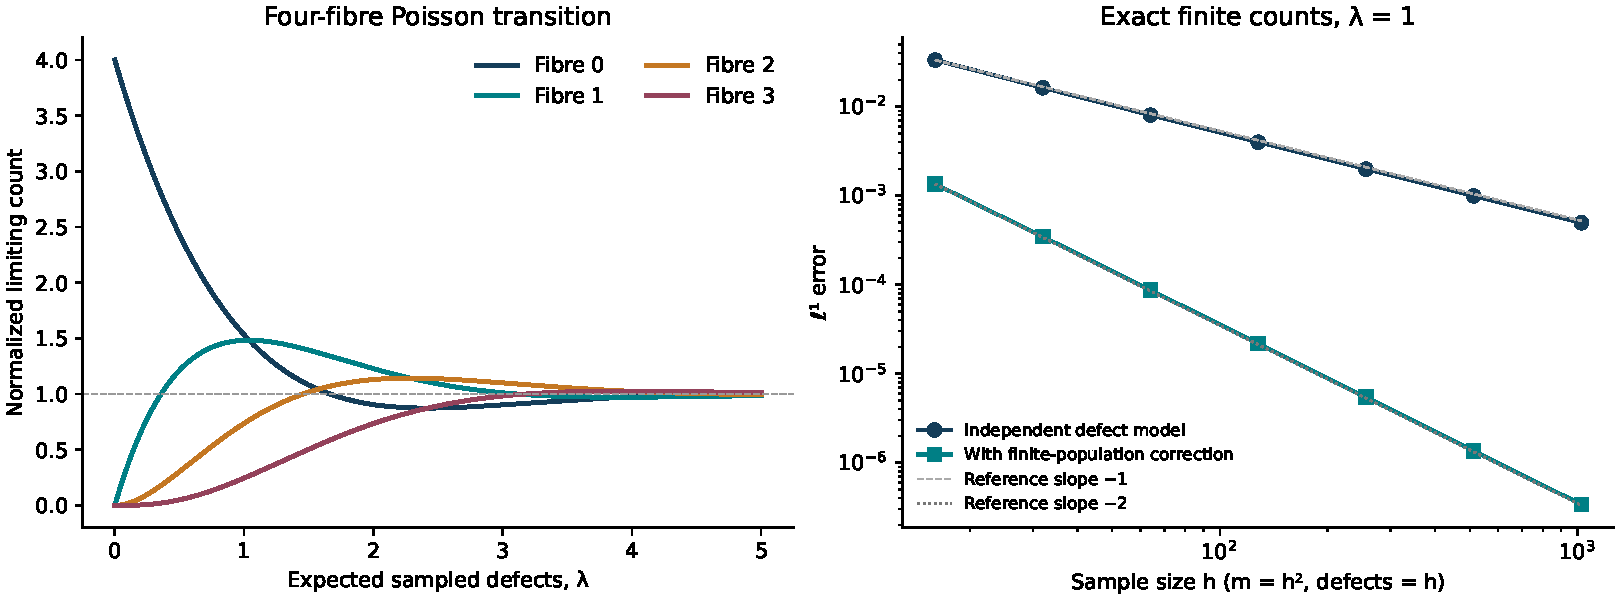
\includegraphics[width=\textwidth]{figures/prime_product_transition.pdf}
\caption{Left: the four normalized densities in the cyclic order-four transition, as given by \eqref{eq:C4}. Right: exact finite-population errors for one defect type, $m=h^2$ and $t=h$, compared with independent Bernoulli inclusion and with the signed correction in \eqref{eq:secondbound}. The displayed slopes illustrate, but do not prove, the orders established analytically.}
\label{fig:transition}
\end{figure}

\subsection*{Reproducible finite verification}
The companion script \texttt{code/verify\_prime\_products.py} uses exact rational arithmetic for finite identities. Its recorded run checked 2,026 population/quota cases against 77,166 independently enumerated subsets, and 44,280 exact coefficient-ratio inequalities. All assertions passed; the results are in \texttt{data/prime\_product\_verification.json}. The script also produces Figure~\ref{fig:transition} and the displayed cyclic-group numerical values. These checks test the finite probability formulas, without constituting a computer proof of the infinite arithmetic statements.

\section{Comparison, significance, and limits}\label{sec:comparison}

The source article already isolates a bounded quotient after arbitrary fixed-density deletions. We retain that reduction and resolve its remaining finite transition law in the sparse regime. Above density $1/4$, the earlier quadratic/cubic criteria are consistent with Theorem~\ref{thm:criterion}. Below that threshold the present criterion includes all character orders at most $D$, while Theorem~\ref{thm:classification} also resolves interactions in noncyclic quotients. It identifies every possible subsequential profile and proves the converse realization, rather than giving only sufficient mixing conditions or exact coefficient formulas. The incoming quarter-density report already solves exact $C_4$ and $C_2^2$ support questions \cite{quarter}; our four-fibre examples concern limiting probabilities. Its independent-exception estimate tends to zero when $t=o(\sqrt m)$. Our critical-window estimate instead gives $O_M(1/h)$ whenever $ht/m\le M$, with no $t=o(\sqrt m)$ restriction, and the signed correction improves the remainder to $O_M(h^{-2})$.

The ordinary relation between hypergeometric and binomial laws is classical; Ehm's Stein--Chen work includes sampling with and without replacement \cite{Ehm}. Higher-order scalar and signed sampling approximations are also classical: L\'opez-Bl\'azquez--Salamanca Mi\~no give Krawtchouk expansions for hypergeometric probabilities \cite{LS}, while Darroch--Ji\v rina--Speed give signed approximations to the full without-replacement sample law \cite{DJS}. The scalar correction mechanism itself is therefore not claimed as new. Poisson laws for prime factors of a random integer are studied, for example, by Ford \cite{Ford}. That model differs from the present uniform fixed-size sample from an adversarially retained small-prime pool. Work of Booker--Pomerance on squarefree smooth representatives \cite{BP}, and more recent work on common short prime sets whose unrestricted subset products cover unit groups \cite{Hughes}, supplies arithmetic context. We do not claim the underlying idea of Poisson approximation, or the source bounded-quotient mechanism, as new.

A targeted check of the supplied article, relevant placed reports, and primary literature did not identify the exact all-density classification and uniform group-algebra expansion proved here. This supports presenting them as candidate research contributions; it does not establish global historical priority or replace expert review. Constants $B,C$ are existential and not optimized. The arithmetic theorem requires $h\ge B\log q$ at the $C\log^2q$ cutoff. No claim is made for shorter quotas, vanishing retained density, or uniformity as $a\to0$. Dense-quota limits have different finite Bernoulli features and are outside the sparse classification. Computations, if supplied with this note, check finite identities and examples; the analytic and asymptotic claims rest on the proofs above.

\begingroup
\raggedright
\begin{thebibliography}{99}
\bibitem{repo} ProveIt contributors, \emph{Generalized Riemann Hypothesis project README}, revision \texttt{6d284fcf75bc3a91bb2e79ba7636f94724bff62c}, 27 November 2026. \url{https://github.com/VladimirReshetnikov/ProveIt/tree/6d284fcf75bc3a91bb2e79ba7636f94724bff62c/Analysis/GeneralizedRiemannHypothesis}.
\bibitem{article} ProveIt contributors, \emph{Beyond the Riemann hypothesis for Dirichlet $L$-functions: consequences, transfers and limits}, same revision, Article/sections/dir.tex, labels cited in Section~1. \url{https://github.com/VladimirReshetnikov/ProveIt/blob/6d284fcf75bc3a91bb2e79ba7636f94724bff62c/Analysis/GeneralizedRiemannHypothesis/Article/sections/dir.tex}.
\bibitem{quadratic} ProveIt research report, \emph{The quadratic-fibre transition for squarefree products of small primes}, 27 November 2026, same revision. \url{https://github.com/VladimirReshetnikov/ProveIt/blob/6d284fcf75bc3a91bb2e79ba7636f94724bff62c/Analysis/GeneralizedRiemannHypothesis/Research/grh_quadratic_fibre/quadratic_fibre.tex}.
\bibitem{quarter} ProveIt research report, \emph{The exact quarter-density obstruction for disjoint products of small primes}, incoming archive \texttt{grh\_quarter\_density.zip}, 27 November 2026, same pinned revision. Its \texttt{quarter\_density.tex}, section on sparse-exception probability profiles, gives the coupling bound compared here. \url{https://github.com/VladimirReshetnikov/ProveIt/tree/6d284fcf75bc3a91bb2e79ba7636f94724bff62c/Analysis/GeneralizedRiemannHypothesis/docs/incoming}.
\bibitem{MV} H. L. Montgomery and R. C. Vaughan, \emph{Multiplicative Number Theory I: Classical Theory}, Cambridge Studies in Advanced Mathematics 97, Cambridge University Press, 2007.
\bibitem{Ehm} W. Ehm, Binomial approximation to the Poisson binomial distribution, \emph{Statistics \& Probability Letters} \textbf{11} (1991), 7--16. \url{https://doi.org/10.1016/0167-7152(91)90170-V}.
\bibitem{LS} F. L\'opez-Bl\'azquez and B. Salamanca Mi\~no, Binomial approximation to hypergeometric probabilities, \emph{Journal of Statistical Planning and Inference} \textbf{87} (2000), 21--29. \url{https://doi.org/10.1016/S0378-3758(99)00187-1}.
\bibitem{DJS} J. N. Darroch, M. Ji\v rina and T. P. Speed, Sampling without replacement: approximation to the probability distribution, \emph{Journal of the Australian Mathematical Society} \textbf{44} (1988), 197--213. \url{https://doi.org/10.1017/S1446788700029785}.
\bibitem{Ford} K. Ford, Joint Poisson distribution of prime factors in sets, \emph{Mathematical Proceedings of the Cambridge Philosophical Society}, published online 23 June 2021. \url{https://www.cambridge.org/core/journals/mathematical-proceedings-of-the-cambridge-philosophical-society/article/abs/joint-poisson-distribution-of-prime-factors-in-sets/524B1FAD27E09853C4A4444E8AEC0ED1}.
\bibitem{BP} A. R. Booker and C. Pomerance, Squarefree smooth numbers and Euclidean prime generators, \emph{Proceedings of the American Mathematical Society} \textbf{145} (2017), 5035--5042. See also the source article's bibliography and its discussion of squarefree small-prime products.
\bibitem{Hughes} S. D. Hughes, \emph{Few small primes suffice to cover unit groups}, arXiv:2610.04678, 2026. \url{https://arxiv.org/abs/2610.04678}.
\end{thebibliography}
\endgroup
\end{document}
